\documentclass{article}

% ready for submission
\usepackage[final]{neurips_2021}
\usepackage[utf8]{inputenc} % allow utf-8 input
\usepackage[T1]{fontenc}    % use 8-bit T1 fonts
\usepackage{hyperref}       % hyperlinks
\usepackage{url}            % simple URL typesetting
\usepackage{booktabs}       % professional-quality tables
\usepackage{amsfonts}       % blackboard math symbols
\usepackage{nicefrac}       % compact symbols for 1/2, etc.
\usepackage{microtype}      % microtypography
\usepackage{xcolor}         % colors
\usepackage{algorithm2e}
\usepackage{amsmath}
\usepackage{graphicx}

\title{CS271 Project: Sokoban Solver}

\author{
  Seokchan Ahn\\
  15288114 \\
  \texttt{seokchaa@uci.edu} \\
   \And
  Youngil Kim\\
  87561931\\
  \texttt{youngik2@uci.edu}\\
   \And
  Jinhwa Kim \\
  86727408 \\
  \texttt{jinhwak@uci.edu}
}
\begin{document}

\maketitle

\begin{abstract}
  Sokoban is a game in which the player pushes boxes around in a warehouse, trying to get them to storage locations. Since the number of possible states can grow exponentially as the board size and number of boxes increase, we suggests model-free reinforcement learning(RL) based solver for this game. Among a variety of RL algorithms, we focus on Monte-Carlo(MC), Temporal-Difference(TD) and Q-learning, which are the most widely used methods.
\end{abstract}

\section{Sokoban}
Sokoban is a game that the user pushes the boxes to the proper storage locations with a minimum number of moves. The map is consists of floor, wall, boxes, and marked storage locations and the above figure shows an example of a state in the Sokoban game. The user can move in 4 directions: Up, Down, Left, Right, and it is not allowed to move through walls or boxes. There are two conditions for terminating the games: 1) All the boxes are on the goals. 2) Deadlocks.

\section{Algorithms}

\subsection{Monte Carlo (MC) Learning}
Monte Carlo Learning method is a way to solve the Reinforcement Learning problem by averaging sample returns. It is a model-free method which means this algorithm does not have knowledge of MDP transition. MC generates episodes and learns from them, but all episodes must terminate.

\RestyleAlgo{ruled}
\begin{algorithm}[H]
\caption{Monte Carlo Learning}\label{alg:one}
\KwData{State $s \in S$ , Action $a \in A(s)= \{U,D,R,L\}$}
Initialize, \par
    \quad Randomly initialize $Q(s,a)$ \par
    \quad $Returns(s,a)$ \gets $\text{empty list}$ \par 
    \quad $\pi$ \gets $\text{random policy}$\par
\While{True}{
    generateEpisode(\pi) \par
    For each pair s,a in episode: \par
        \quad Q(s,a) \gets average(R(s,a)) \par
    For each s in the episode: \par
        \quad a* \gets argmax(Q(s,a)) \par
        \quad For all $a \in  A(s)$: \par
        \quad\quad \pi(s,a) \gets $\text{epsilon-soft policy update}$ \par
}
\SetAlgoLined
\SetKwProg{Fn}{Function}{is}{end}
\Fn{generateEpisode(\pi,numberOfepisodes)}{
episodes \gets \text{empty list}\par
\While{ $n < numberOfepisodes$}{
    timestamp \gets \text{empty list}\par
    \While{not goalSate()}{
    $\text{Get}$ $s, a ,r$ depending on policy \par
    $\text{Append}$ $s, a ,r$  to timestamp \par
    }
    $\text{Append}$ timestamp to episodes \par
    n \gets n+1 \par
}}
\end{algorithm}

\textit{Policy Evaluation} \par
The Monte Carlo Learning method does not have a model. Thus, this model uses the mean of return of samples for evaluating policy instead of the expected return as Bellman expectation backup does. 


\textit{Problem} \par
Because MC learning initializes policy randomly, it could take a quite long time to make a terminate episode. It means that while loop part falls in infinite iterations.
Thus, We can use Temporal Difference(TD) learning or update policy on the partial completed state, not the complete end state.


\subsection{Temporal Difference(TD) Learning}
Temporal Difference is also one of model-free reinforcement learning methods, but most difference from MC methods comes from the fact that it does not necessarily require complete episodes, so it takes advantage of MC methods and Dynamic Programming (DP) methods by bootstrapping from the current estimate of the value function. In TD learning, the algorithm samples from the environment like MC methods, but performs updates based on current estimates like DP methods.

In TD Learning, we should consider 4 hyperparams; $\gamma$, $\lambda$, $\alpha$, and $\delta$. $\gamma$ is the discount rate, which is a value between 0 and 1. The higher the value the less you are discounting.  $\lambda$ is the credit assignment variable, which is also a value between 0 and 1. The higher the value the more credit you are able to assign to further back states and actions. $\alpha$ is the learning rate, showing how much of the error should we accept and adjust our estimates towards. Lastly, $\delta$ is a change in value. In our approach, we are planning to choose $\lambda$ is 0 for simplicity and efficiency.

% \RestyleAlgo{ruled}
% \SetKwComment{Comment}{/* }{ */}
% \begin{algorithm}[H]
% \caption{TD(0) Learning}\label{alg:td}
% \SetAlgoLined
% \KwData{the policy $\pi$ to be evaluated
% }
%  Initialize $V(s)$\;
%  \For{each episode}{
%   Initialize $s$\;
%   Initialize $step$, $maxStep$\;
%   \While{$step$ \leq $maxStep$}{
%     $A \gets getAction(\pi, S)$\Comment*[r]{get Action from policy \pi}
%     $V(S) \gets V(S)+\alpha[R+\gamma V(S') - V(S)]$\Comment*[r]{update $V(S)$} 
%     $S \gets S'$\Comment*[r]{update current state}
%     \If{$isGoalState(s')$} {
%       break\Comment*[r]{arrived to one of the goal states}
%   }
%   $step \gets step + 1$\Comment*[r]{increase current step by 1}
%   }
%  }
% \end{algorithm}

\subsection{Q-Learning}

Q-learning is a model-free reinforcement learning algorithm to learn the value of an action in a particular state. It is an off-policy learning because the executed actions are different from the target actions that are used for learning. It updates values based on the next state's best action, but choose the action by $\epsilon$-greedy policy, which enables both exploration and exploitation.

\begin{algorithm}[H]
\caption{Q-Learning}\label{alg:one}
\KwData{State $s \in S$ , Action $a \in A(s)= \{U,D,R,L\}$}
Initialize $Q(S, A)$ as zero\;
Initialize $maxStep, \epsilon, \alpha, \gamma$\;
Initialize $s$ \Comment*[r]{initial state}
$step \gets 1$\;

\While{$step \leq maxStep$}{
  $a \gets getAction(s, \epsilon)$ \Comment*[r]{choose action using $\epsilon$-greedy policy}
  $s', r \gets getNextState(action)$ \Comment*[r]{next state, reward}
  $Q(s, a) \gets Q(s, a) + \alpha(r + \gamma \max Q(S', a) - Q(s, a))$ \Comment*[r]{update Q for s, a}
  $s \gets s'$ \Comment*[r]{update state to new state}

  \If{$isTerminal(s')$)} {
    Initialize $s$ \Comment*[r]{start over from the initial state}
  }
  $step \gets step + 1$\Comment*[r]{increase current step by 1}
}
\end{algorithm}

There are three hyperparams in Q-learning. First, $\epsilon$ decides the possibility of exploitation. In general, $\epsilon$ is initialized as 1.0, which means the agent will choose a random action with a probability of 1.0, since there is no information about the expected value in the beginning. As the estimated Q-values converge, $\epsilon$ should be decayed to exploit the learned values. $\alpha$ and $\gamma$ are the learning rate and the discount rate by time for each.

\begin{algorithm}[H]
\caption{Q-Learning Inference}\label{alg:two}
\KwData{State $s \in S$ , Action $a \in A(s)= \{U,D,R,L\}$}
Initialize $s$ \Comment*[r]{initial state}
$\epsilon \gets 0.0$ \Comment*[r]{greedy policy}

\While{$True$}{
  $a \gets getAction(s, \epsilon)$ \Comment*[r]{choose action using $\epsilon$-greedy policy}
  $s', r \gets getNextState(action)$ \Comment*[r]{next state, reward}
  $s \gets s'$ \Comment*[r]{update state to new state}
  \If{$isGoalState(s')$} {
    break \Comment*[r]{Arrived to one of the goal states}
  }
}
\end{algorithm}

In the inference time, the agent can greedy choose the best action at the current state every time. It can be done by simply using the $\epsilon$ value of zero.



\section{Implementation Details}

\subsection{States and Actions}

In the Sokoban game, states can be defined as the setting of the board. Since the positions of walls and storages are fixed, we can use the coordinations of the boxes and the player as a state. Since the order of boxes doesn't matter, we use a hash map for Q-table using `(set(boxes), player)` as keys and Q-values as values. For actions, we use `[L, U, R, D] since they are all the available movements.

A Sokoban game's terminal states are 1) when all the boxes are on the goals, or 2) when on a Deadlock state.

\subsubsection{Deadlocks}

\paragraph{Simple deadlocks}
A simple deadlock is created by moving just one box to border lines, which makes it unable to reach any goal state, no matter what the agent moves. In the figure \ref{fig:simple}, pushing the box to a darker shaded space results in a simple deadlock.

\paragraph{Freeze deadlocks}
Freeze deadlocks refer to the situation that all boxes become immovable. If a box becomes immovable while not being located on a goal, the game is deadlocked. In the figure \ref{fig:freeze}, pushing the box one square up results in a freeze deadlock.

\paragraph{Corral deadlocks}
Corral indicates a zone that the agent cannot access. Corral deadlocks can be created when deadlock happens if the agent is not able to move the box because of presence of corral. In the figure \ref{fig:corral}, marked area with little blue quadrats is a corral, and it is not reachable for the agent. Pushing the lower box to the right square results in a corral deadlock.

\begin{figure}
\centering
\begin{minipage}[b]{4cm}
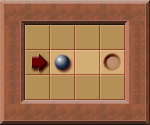
\includegraphics[width=4cm]{SimpleDeadlockExample.png}
\caption{Simple Deadlock}
\label{fig:simple}
\end{minipage}
\begin{minipage}[b]{4cm}
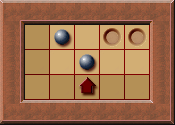
\includegraphics[width=4cm]{FreezeDeadlockExample.png}
\label{fig:freeze}
\caption{Freeze Deadlock}
\end{minipage}
\begin{minipage}[b]{4cm}
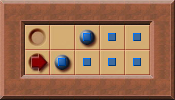
\includegraphics[width=4cm]{CorralDeadlockExample.png}
\label{fig:corral}
\caption{Corral Deadlock}
\end{minipage}
\end{figure}

\subsection{Rewards}
Rewards are the most important part in reinforcement learning since it decides which actions are good or bad and how good or bad they are. We defined the categories of rewards as below.

% Please add the following required packages to your document preamble:

\begin{table}[h]
\centering
\resizebox{\textwidth}{!}{%
\begin{tabular}{|l|l|p{8cm}|}
\hline
Category          & Reward & Description                                                                                                                         \\ \hline
MOVE              & -0.1   & To prevent looping infinitely, give small penalty for each move                                                                     \\ \hline
BOX\_ON\_STORATE &
  1.0 &
  Since it may takes too many steps to the final goal, updating Q-values from the final reward is difficult. Therefore, giving rewards for achieving intermediate goals can make the Q converge faster. \\ \hline
BOX\_OFF\_STORAGE & -1.0   & Give penalty for pushing a box away from a storage.                                                                                 \\ \hline
ALL\_ON\_STORAGE  & 10.0   & Give reward when the player successfully finishes the game.                                                                         \\ \hline
DEADLOCK          & -10.0  & Once it gets to a deadlock state, it can never be solved afterwards. Therefore, give a great penalty and initialize the state again. \\ \hline
MOVE\_TO\_WALL    & -1.0   & Trying to go toward a wall or a box in front of another box or a wall is not worth. Therefore, give a small penalty.                \\ \hline
\end{tabular}%
}
\caption{Categories of rewards and their values}
\label{tab:rewards}
\end{table}




% \appendix

% \section{Appendix}

% Optionally include extra information (complete proofs, additional experiments and plots) in the appendix.
% This section will often be part of the supplemental material.

\end{document}